%---------------------------------------------------------------
% File information.

% Filename : docs/requirements.tex
% Purpose  : Multiplayer, networked Checkers game for CS451.
% Authors  : Corwin Belser <cmb539@drexel.edu>
%            Zach Brennan  < zab37@drexel.edu>
%            Kris Horsey   < kth37@drexel.edu>
%            Zach van Rijn < zwv23@drexel.edu>
% License  : MIT/X (excl. ext. libs; see respective licenses).
% Revision : 20170805

%---------------------------------------------------------------
% README.

% This is currently a DRAFT.
%
% Also please keep it to NO MORE THAN 64 columns. This isn't a
% requirement by LaTeX, but a guideline we are following for the
% entire project. Thanks.
%
% You will need some kind of LaTeX compiler. Recommend this:
% https://www.tug.org/texlive/acquire-netinstall.html
% which works on Windows and Linux.
%
% The `vhistory' package has nice documentation:
% http://mirrors.rit.edu\
% /CTAN/macros/latex/contrib/vhistory/doc/vh_sets_en.pdf
%
% And this page on making tables:
% https://en.wikibooks.org/wiki/LaTeX/Tables

%---------------------------------------------------------------
% Includes.

\documentclass[letterpaper]{article}

\usepackage[english]{babel}
\usepackage[useregional]{datetime2}
\usepackage{hyperref}                   % \url
\usepackage{cleveref}                   % \cref
\usepackage{bookmark}                   % tracks .out files
\usepackage{vhistory}                   % for version history
\usepackage{subcaption}                 % for nested figures
\usepackage{listings}                   % \lstlisting, \lstset
\usepackage{amssymb}                    % for keyword styling
\usepackage[usenames,dvipsnames]{color} % for colors
\usepackage{courier}                    % \ttfamily
\usepackage{tabulary}                   % \tabulary (more flex.)
\usepackage[numbers, square]{natbib}    % for proper \bibsection

\usepackage{tikz}                       % for dem ol' shapez!
\usetikzlibrary{shapes.geometric, arrows}

%---------------------------------------------------------------
% Macros.

% Produces a sexy table for pre- and post-conditions.
\newcommand{\prepost}[3]
{
    \begin{tabulary}{\linewidth}{p{2.5cm}p{7.5cm}}
    \textbf{Precondition}:  & #1\\\\
    \textbf{Action}:        & #2\\\\
    \textbf{Postcondition}: & #3\\
    \end{tabulary}
}

%\newcommand{\prepost}[5]
%{
%    \begin{tabulary}{\linewidth}{p{#1}p{#2}}
%    \textbf{Precondition}:  & #3\\\\
%    \textbf{Action}:        & #4\\\\
%    \textbf{Postcondition}: & #5\\
%    \end{tabulary}
%}

%---------------------------------------------------------------
% Listings.

% https://tex.stackexchange.com/questions\
% /31328/how-to-typeset-data-structures

% define a pseudocode language
\lstdefinelanguage{algpseudocode}
{
    keywordstyle=[1]{\keywordstyle},
    keywordstyle=[2]{\operatorstyle},
    keywordstyle=[3]{\typestyle},
    keywordstyle=[4]{\functionstyle},
    identifierstyle={\identifierstyle},
    keywords=[1]{%
    begin,end,%
    program,procedure,function,subroutine,%
    while,do,for,to,next,repeat,until,loop,%
    continue,endwhile,endfor,endloop,%
    if,then,else,endif,%
    return},
    literate={-}{$-$}1 {^}{$^\wedge$}1
    {>}{{$>$\ }}1 {<}{{$<$\ }}1
    {>=}{{$\geqslant$\ }}1 {<=}{{$\leqslant$\ }}1 
    {:=}{{$\gets$\ }}1 {!=}{{$\ne$\ }}1 {<>}{{$\ne$\ }}1
    {->}{{$\;\to\;$}}1
    {&&}{{\keywordstyle and\ }}4 {{||}}{{\keywordstyle or\ }}3
    {;}{\hspace{0.2em};}2 {,}{\hspace{0.2em},}2,
}

% some macros to fine-tune styles
\newcommand\keywordstyle{\rmfamily\bfseries\upshape}
\newcommand\operatorstyle{\rmfamily\mdseries\upshape}
\newcommand\typestyle{\rmfamily\mdseries\upshape}
\newcommand\functionstyle{\rmfamily\mdseries\scshape}

\newcommand\identifierstyle{\rmfamily\mdseries\itshape}

\newcommand\addkeywords[1]{%
    \lstset{morekeywords=[1]{#1}}}

\newcommand\addoperators[1]{%
    \lstset{morekeywords=[2]{#1}}}

\newcommand\addtypes[1]{%
    \lstset{morekeywords=[3]{#1}}}

\newcommand\addfunctions[1]{%
    \lstset{morekeywords=[4]{#1}}}

\definecolor{Brown}{cmyk}{0,0.81,1,0.60}
\definecolor{OliveGreen}{cmyk}{0.64,0,0.95,0.40}
\definecolor{CadetBlue}{cmyk}{0.62,0.57,0.23,0}
\definecolor{gray}{cmyk}{0,0,0,0.5}

%---------------------------------------------------------------
% Shapes.

% Should probably come up with new shapes.

\tikzstyle{startstop} = [
    rectangle,
    rounded corners,
    minimum width=3cm,
    minimum height=1cm,
    text centered,
    draw=black,
    fill=red!30
]

\tikzstyle{io} = [
    trapezium,
    trapezium left angle=70,
    trapezium right angle=110,
    minimum width=3cm,
    minimum height=1cm,
    text centered,
    draw=black,
    fill=blue!30
]

\tikzstyle{process} = [
    rectangle,
    minimum width=3cm,
    minimum height=1cm,
    text centered,
    text width=3cm,
    draw=black,
    fill=orange!30
]

\tikzstyle{decision} = [
    diamond,
    minimum width=3cm,
    minimum height=1cm,
    text centered,
    draw=black,
    fill=green!30
]

% Arrows.

\tikzstyle{arrow} = [thick,->,>=stealth]
\tikzstyle{conns} = [thick,-,>=stealth]

%---------------------------------------------------------------
% Configuration.

\renewcommand{\thefootnote}{\arabic{footnote}}

\title{
    Console-Based Checkers Game\\
    Requirements Specifications
    \footnote{CS451:002 Group 2, Drexel University}
}

% \usepackage{authblk} causes problems with alignment, though it
% also allows us to properly include affiliations.. pick poison.
\author{
    Belser, C.\\
    \texttt{cmb539@drexel.edu}
    \and
    Brennan, Z.\\
    \texttt{zab37@drexel.edu}
    \and
    Horsey, K.\\
    \texttt{kth37@drexel.edu}
    \and
    van Rijn, Z.\\
    \texttt{zwv23@drexel.edu}
}

\date{\today}

%---------------------------------------------------------------
% Document begin.

\begin{document}

%---------------------------------------------------------------
% Header.

\maketitle

\begin{abstract}

The game \emph{Checkers}, also known as \emph{Draughts}
\footnote{\url{https://en.wikipedia.org/wiki/Draughts}}, is a
turn-based game playable by all ages. This document outlines the
requirements for a console-based software implementation of the
game, which allows players to enjoy the game from any Internet-
connected computer.

\end{abstract}

%---------------------------------------------------------------
% Table of Contents.

\tableofcontents
\newpage

%---------------------------------------------------------------
% Revision History.

\begin{versionhistory}
    \vhEntry{0.90}
        {\date{\DTMdisplaydate{2017}{07}{22}{-1}}}
        {ZV}
        {created \LaTeX~skeleton}
    \vhEntry{0.91}
        {\date{\DTMdisplaydate{2017}{07}{22}{-1}}}
        {ZV}
        {added platform specifications}
    \vhEntry{0.92}
        {\date{\DTMdisplaydate{2017}{07}{30}{-1}}}
        {ZV}
        {added remarks about Docker, others}
    \vhEntry{0.93}
        {\date{\DTMdisplaydate{2017}{08}{01}{-1}}}
        {CB}
        {added to Client Functionality \& User Interface}
    \vhEntry{0.94}
        {\date{\DTMdisplaydate{2017}{08}{04}{-1}}}
        {KH}
        {added Glossary \& updated user interface and 
        introduction}
    \vhEntry{0.95}
        {\date{\DTMdisplaydate{2017}{08}{05}{-1}}}
        {ZV}
        {added pseudocode, server logic, others}
    \vhEntry{0.96}
        {\date{\DTMdisplaydate{2017}{08}{05}{-1}}}
        {ZB}
        {added to Non-Functional Requirements}
    \vhEntry{0.97}
        {\date{\DTMdisplaydate{2017}{08}{05}{-1}}}
        {CB}
        {added detail to Client Functionality \& User 
        Interface Requirements}
    \vhEntry{0.98}
        {\date{\DTMdisplaydate{2017}{08}{06}{-1}}}
        {ZV}
        {added charts}
    \vhEntry{0.99}
        {\date{\DTMdisplaydate{2017}{08}{06}{-1}}}
        {(all)}
        {finished documentation}
    \vhEntry{1.00}
        {\date{\DTMdisplaydate{2017}{08}{06}{-1}}}
        {(all)}
        {\textbf{final team approval}}
\end{versionhistory}
\newpage

%---------------------------------------------------------------
% Introduction.

\section{Introduction}
\label{sec:intro}

\subsection{Purpose of Document}
\label{sec:intro_purpose}

This document shall serve as a reference for all current and
future software developers and project managers affiliated with
this project. These specifications are considered contractual,
and all functionality must be implemented in accordance to this
document. Additional or modified functionality is permissible
only where explicitly stated. This document will also function
as a reference for the evaluator.

\subsection{Document Conventions}
\label{sec:intro_conventions}

Content is organized in a sequential hierarchical manner. We
aim to provide high-level descriptions and further elaborate
in later sections. We may write console commands
\texttt{like this}. We may refer to applications, tools,
libraries, or other dependencies \emph{like this}. These are
often followed by some sort of citation, via which the reader
may seek additional information.

Generally, we try to follow the IEEE Software Requirements
Specification \texttt{ISO/IEC/IEEE 29148:2011}~\cite{ieeesrs}
guidelines, however elements of older standards may have made
it into this document.

\subsection{Intended Audience and Reading Suggestions}
\label{sec:intro_audience}

The intended audience of this document is computer scientists
who have interest  in seeing the components that go into the
team's implementation of the game of Checkers in the C
language. The document uses official tournament rules for the
game of checkers therefore some rules might be unfamiliar for
those who haven't played or observed checkers at a competitive
level.

\subsection{Scope of Document}
\label{sec:intro_scope}

We thoroughly detail the complete software requirements so that
any software development team may follow, develop, and test the
software. This document will detail the intended behavior and
expected interactions between each component.

\subsection{Overview of Document}
\label{sec:intro_overview}

Graphical figures, tables, and code listings are commonly used
in addition to textual descriptions to convey the intent, logic,
and desired functionality to a person or persons unfamiliar with
the project. We therefore include such elements with the hope
that it better conveys our requirements, however we cannot make
any guarantee that such figures will be effective. If there are
any questions, about any of the material contained within this
document, please do not hesitate to contact one of the authors.

\subsection{Project Scope}
\label{sec:intro_project}

This document describes the high-level user requirements and
specifications for a console-based Checkers implementation. The
goal of the software is to provide an intuitive client where the
users can comfortably play the game of Checkers. Specifically:

\begin{enumerate}
    \item Automatic ``move'' validation, where player(s)' moves
          will be validated in realtime against a predefined set
          of official Checkers rules
    \item Ability to play the game on several Unix-like systems
    \item Provide exemplary source code quality that can be used
          as a teaching tool
\end{enumerate}

We will consider the following to be \emph{nice-to-have}'s, or
features that we would like to implement but cannot guarantee to
be included in the final deliverable:

\begin{enumerate}
    \item Client Spectators~\cref{sec:fun_reqs_client_spectator}
          to allow additional clients to connect to the game
          server for the sole purpose of watching an existing
          game
    \item Web-based implementation, which may run natively as
          compiled WebAssembly\cite{webassembly} or via an
          intermediate server and accessed via a VNC~\cite{vnc}
          client
\end{enumerate}

%---------------------------------------------------------------
% Description.

\section{Overall Description}
\label{sec:description}

This document describes the complete requirements for a console-
based implementation of the game \emph{Checkers}. Slight changes
may be present between the original game and the console-based
implementation (hereforth known as \textbf{game}). Therefore, it
is imperative that the product description be read, understood,
and any confusion clarified, by all parties, before development
begins.

The \textbf{game} is a two player game designed to be played
remotely (by two computers on joint or disjoint networks). When
a player joins the game they are taken to a waiting screen until
a second player has joined. Once two players are connected, they
are taken to a checker game board and begin the game. Players
then take turns making moves until either a draw is reached
(neither play can force a win), when one player has no pieces
remaining on the board, or if a player has no legal moves 
available on their turn. At this point a winner is displayed 
(or that it was a draw) and the game concludes.

The game will require a server and two or more connected clients
where any additional clients become \emph{spectators}.

\subsection{Product Perspective}
\label{sec:description_product}

The \textbf{game} is typically played on a square checkboard of
dimensions \emph{8x8}, though several variations\footnote{
    English draughts (8x8) a.k.a. American Checkers,
    Russian draughts (8x8),
    International (Polish) draughts (10x10),
    Canadian checkers (12x12)~\cite{draughts}
} exist, we will focus on the \emph{American checkers} variety.

\subsection{Game Rules}
\label{sec:description_rules}

This version of the game has the following rules~\cite{rules},
modified for formatting:

\begin{enumerate}
    \item Checkers is played by two players. Each player begins
          the game with 12 colored discs. (Typically, one set of
          pieces is white and the other red.)
          
    \item The board consists of 64 squares, alternating between
          32 dark and 32 light squares. It is positioned so that
          each player has a light square on the right side
          corner closest to him or her.

    \item Each player places their pieces on the 12 dark squares
          closest to them.
          
    \item White moves first. Players then alternate moves.
    
    \item Moves are allowed only on the dark squares, so pieces
          always move diagonally. Single pieces are always
          limited to forward moves (toward the opponent).
          
    \item A piece making a non-capturing move (not involving a
          jump) may move only one square.
          
    \item A piece making a capturing move (a jump) leaps over
          one of the opponent's pieces, landing in a straight
          diagonal line on the other side. Only one piece may be
          captured in a single jump; however, multiple jumps are
          allowed during a single turn.
          
    \item When a piece is captured it is removed from the board.
    
    \item If a player is able to make a capture, there is no
          option -- the jump must be made. If more than one
          capture is available, the player is free to choose
          whichever they prefer.
          
    \item When a piece reaches the furthest row from the player
          who controls that piece, it is crowned and becomes a
          king. One of the pieces which had been captured is
          placed on top of the king so that it is stacked twice
          as high.

    \item Kings are still limited to moving diagonally, but may
          move both forward and backward. (Remember that single
          pieces, i.e. non-kings, are always limited to forward
          moves.)
          
    \item Kings may combine jumps in several directions --
          forward and backward -- on the same turn. Single
          pieces may shift direction diagonally during a
          multiple capture turn, but must jump forward (toward
          the opponent).

    \item A player wins the game when the opponent cannot make a
          move. In most cases, this is because all of the
          opponent's pieces have been captured, but it could
          also be because all of their pieces are blocked in.
\end{enumerate}

\subsection{Product Features}
\label{sec:description_features}

As a complete system, our product is composed of several smaller
subsystems.



\subsubsection{Server}
\label{sec:description_product_server}

The server will act as the main driver for the game, controlling
player connections, dictating player turns,updating the board,
checking win-state, and providing updatedgame-states to the
clients.

\subsubsection{Client}
\label{sec:description_product_client}

The client will act as the player interface, displaying the game
to the player, gathering player moves, and displaying messages
from the server. A client can be instructed (by the server) to
operate in a reduced-functionality mode, where such a client is
unable to make moves, and therefore functions as a spectator to
the current, active game.

\subsection{User Classes and Characteristics}
\label{sec:description_user}

Typical users for \textbf{game} are the same who enjoy the
traditional board game, and individuals who may not be familiar
with the game. The rules are straightforward, and anyone with a
computer and an Internet connection should be able to learn,
play, and hone their skills in this competitive, thrilling new
console environment. Some users may even find a bit of nostalgia
in our rendition of the classic game.

\subsection{Operating Environment}
\label{sec:description_environment}

Docker~\cite{docker} is a software platform that abstracts many
aspects of the operating system in order to provide an isolated
environment, called a `container', which may contain only the
bare minimum required libraries and packages to support a given
application. The filesystem, network interfaces, and other parts
of the host system are available to the container as needed, and
while it shares a common kernel with other adjacent containers,
it does not depend on the host system for any other libraries.

We recommend using Docker as a platform for both building and
initial testing of the software. We have provided an image that
closely resembles our internal computing envrironment, based on
\texttt{alpine:3.6}, a minimal Unix-like environment. The image
we provide has several tools and libraries preinstalled, which
can be linked statically to produce a portable executable for
distribution to end-users, further described in
\cref{sec:description_dependencies}.

\subsection{Design Constraints}
\label{sec:description_constraints}

There are no relevant regulatory or financial constraints that
should be considered at this time.

The product may have external dependencies, which are described
in \cref{sec:description_dependencies}. These dependencies have
been captured in a ``frozen'' state (stable releases) to avoid
future complications and compatibility issues. Copies of these
dependencies are stored on a common project server to mitigate
issues in the event that those projects become unavailable.

\subsection{User Documentation}
\label{sec:description_documentation}

Complete user documentation, including usage manuals and setup
guides will be available at the following URL at the conclusion
of the project:\\\url{https://git.zv.io/me/CS451-Checkers}. We
may publish final PDF versions at a different URL, which may be
found in one of the Appendices of this document, if available.

\subsection{Assumptions}
\label{sec:description_assumptions}

In order to guarantee that the software builds and runs on an
agreed-upon generic platform, and operates correctly, we define
the minimum expected software and hardware configuration that
must be supported by the application. In other words, the game
should be playable with the minimum specifications, but it can
be assumed that most users will have machines that at least
meet or exceed the ``ideal'' hardware and/or software.

\begin{figure}
    \centering
    \begin{subfigure}{.50\textwidth}
        \centering
        \begin{tabulary}{\linewidth}{LCC}
            Component & Min.    & Ideal    \\
            \hline
            CPU       & 200 MHz & 1.0 GHz  \\
            Memory    &  64 MB  & 256 MB   \\
            Disk      & 500 MB  & 1.0 GB   \\
            Display   & 800x600 & 1024x768 \\
        \end{tabulary}
        \caption{Hardware}
        \label{fig:description_assumptions_hard}
    \end{subfigure}%
    \begin{subfigure}{.50\textwidth}
        \centering
        \begin{tabulary}{\linewidth}{LLL}
            Component & Min.   & Ideal  \\
            \hline
            kernel    & 2.6.32 & 4.4.0  \\
            make      & 3.82   & 4.1    \\
            gcc       & 4.8.4  & 5.4.0  \\
            bash      & 4.2.46 & 4.3.48 \\
        \end{tabulary}
        \caption{Software}
        \label{fig:description_assumptions_soft}
    \end{subfigure}
    \caption{Generic System Requirements}
    \label{fig:description_assumptions}
\end{figure}

\subsubsection{Hardware}
\label{sec:description_assumptions_hard}

Figure \cref{fig:description_assumptions_hard} contains minimum
and ideal specifications of a generic platform that should be
able to operate the game. This does \emph{not} necessarily mean
it needs to be able to compile (build the game), but the ideal
specifications should be sufficient to do so.

\subsubsection{Software}
\label{sec:description_assumptions_soft}

Figure \cref{fig:description_assumptions_soft} contains minimum
and ideal specifications of a generic platform that should be
able to operate the game. This does \emph{not} necessarily mean
it needs to be able to compile (build the game), but the ideal
specifications should be sufficient to do so.

\subsection{Dependencies}
\label{sec:description_dependencies}

Most or all of the software dependencies are directly satisfied
or satisfied by equivalent packages in the first stage of the
project prototype.

\subsubsection{Essential Libraries}
\label{sec:description_dependencies_essential}

These libraries are automatically pulled into the project and
used during the compilation of the game. They should be built
and linked statically, such that the final executable can be
transferred to any supporting system for immediate use.

\begin{enumerate}
    \item \emph{musl}, a lightweight libc implementation
          ~\cite{musl}
    \item \emph{ncurses}, a text-based user-interface API
          ~\cite{ncurses}
    \item \emph{check}, a unit-testing framework for C
          ~\cite{check}
    \item \emph{freetype}, a font parsing library for C
          ~\cite{freetype}
\end{enumerate}

\subsubsection{Supplemental Tools}
\label{sec:description_dependencies_supplemental}

Some additional tools can be built, optionally, to aid in the
process of debugging and testing to ensure the application works
in a safe manner.

\begin{enumerate}
    \item \emph{cppcheck}, a static analysis tool for C and C++
          ~\cite{cppcheck}
    \item \emph{valgrind}, a suite of debugging tools
          ~\cite{valgrind}
\end{enumerate}

%---------------------------------------------------------------
% External Interface Requirements.

\section{External Interface Requirements}
\label{sec:iface_reqs}

\subsection{User Interfaces}
\label{sec:iface_reqs_user}

The user will be presented with an 8x8 Checkerboard initially
containing all of the pieces for a game of Checkers. The
user will interact with the environment through the use
of a cursor that highlights the currently selected square. The
squares with legal moves for that player will be highlighted and
once the user makes their selection they will confirm their move
using the \texttt{enter} key.

\subsection{Hardware Interfaces}
\label{sec:iface_reqs_hardware}

\emph{No special hardware interfaces are required}.

\subsection{Software Interfaces}
\label{sec:iface_reqs_software}

\emph{No special software interfaces are required}.\\

If time permits, game move validator API could be standardized
to serve as a standalone tool or simple network service that can
be used by the general public for any Checkers-related purposes.

\subsection{Communications Interfaces}
\label{sec:iface_reqs_comms}

The interface for client-server communication shall consist of
the following pseudocode:

% define 'algpseudocode' listing settings
\lstset{%
    language={algpseudocode},
    columns=fullflexible,
    numbers=left,
    numberstyle=\scriptsize,
}

\addfunctions{AcceptClient}
\addfunctions{BeginGame}
\addfunctions{listen_tcp}
\addfunctions{Listening}
\addoperators{send,receive,READY,false,close_tcp}
\addoperators{connection,start_port,id}
\addoperators{max_clients}

\begin{figure}
    \begin{lstlisting}
    :: move connected client to a dedicated port
    :: players with id > 2 will be spectators
    
    procedure AcceptClient(connection, start_port, id)
        send(connection, id, start_port + id)
        if receive(connection, start_port + id) == READY
            return BeginGame() :: not shown
        end if
        return false :: kills the thread
    end procedure

    :: max_clients: at least 2; higher to accommodate spectators
    :: start_port : 1024 < start_port < 65535
    
    procedure Listening(max_clients, start_port)
        id := 0
        while listen_tcp(start_port)
            if connection && id != max_clients
                if AcceptClient(connection, start_port, id + 1)
                    id++
                else
                    send(connection, false, 'You must be ready')
                    close_tcp(connection)
                end if
            else
                send(connection, false, 'Server is full')
            end if
        end while
    end procedure
    \end{lstlisting}
    \caption{Server Logic for New Connections}
    \label{fig:iface_reqs_comms_server}
\end{figure}

%---------------------------------------------------------------
% Functional Requirements.

\section{Functional Requirements}
\label{sec:fun_reqs}

\subsection{System Features}
\label{sec:fun_reqs_system}

The system will give users the option to create a new game,
allow them to join a game, or allow them to participate as a
spectator in an ongoing game. The system will also have an
options menu that will allow users to change aspects of the game
such as the length of each turn.

\subsection{Server Functionality}
\label{sec:fun_reqs_server}

High-level logic for how the server component should behave is
defined in \cref{fig:iface_reqs_comms_server}. Implementation
details are intentionally omitted; they will be part of the
design document, \texttt{design.pdf}. The server should always
accept new connections, but reject connections if it is ``full''
or if the client does not respond appropriately.

\begin{figure}
    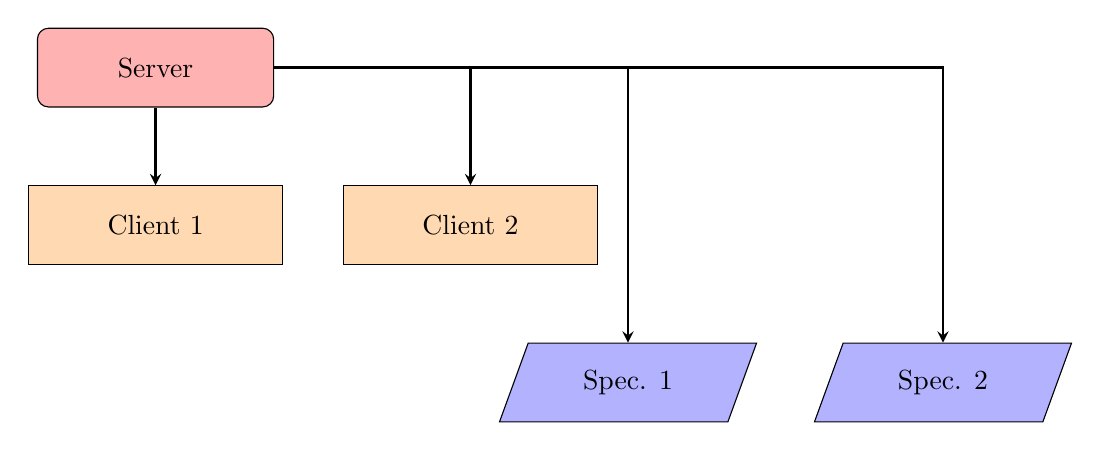
\begin{tikzpicture}[node distance=2cm]
    \node (server) [startstop] {Server};
    \node (client_a) [process, below of=server] {Client 1};
    \node (client_b) [process, right of=client_a, xshift=2cm] {Client 2};
    \node (spects_a) [io, below of=client_b, xshift=2cm] {Spec. 1};
    \node (spects_b) [io, right of=spects_a, xshift=2cm] {Spec. 2};

    \draw [arrow] (server) -- (client_a);
    \draw [arrow] (server) -| (client_b);
    \draw [arrow] (server) -| (spects_a);
    \draw [arrow] (server) -| (spects_b);
    \end{tikzpicture}
    \caption{Server-Client Hierarchy, Spectators Optional}
    \label{fig:diagrams_sch}
\end{figure}

\subsubsection{Client Connections}
\label{sec:fun_reqs_server_client}

\begin{enumerate}
    \item \textbf{Accept connections from clients}
    
          The server shall enter a \emph{listening} state in
          which it listens for TCP connections on a specified
          port. Usage might be as follows:\\
          \newline
          \texttt{./server --base-port 9000 --max-clients 5}
          \newline
          
    \item \textbf{Pair first two client connections into a game}
    
          While the server is listening for new connections, it
          shall treat the \emph{first} successfully-connected
          client as \emph{Player 1}, and the \emph{second}
          as \emph{Player 2}. Further connections, if allowed,
          will become \emph{spectators}. Each player will be
          notified of their \emph{id}, an integer in the range
          \texttt{1 < id < max-clients}. Each client will be
          redirected to a new port, which is calculated in the
          following manner:\\
          \newline
          \texttt{port = base\_port + id}
          \newline
       
          Once the first two clients have connected, the server
          initiates a new game, constructing an internal board
          state and performing other necessary steps.
          
    \item \textbf{Premature client disconnection}
    
          In the event that a client disconnects prematurely,
          defined as:
          
          \begin{enumerate}
              \item the network connection is dropped for any
                    reason
              \item the client chooses to close the application
                    before the game is completed
          \end{enumerate}
          
          The server will notify the opponent that they are the
          winner of the game, then perform the following steps:
          
          \begin{enumerate}
              \item clean up the current game state
              \item ask the winner if they would like to
                    continue playing the game (as in, start a
                    new game)
              \item ask the first-connected spectator (if
                    available) whether they would like to play a
                    game, moving to each successive spectator
                    until an agreement has been reached
              \item if no spectators are available, the game
                    will wait for a new connection, in similar
                    fashion to how it starts initially
              \item if the winner chooses \emph{not} to continue
                    then all client(s) are immediately
                    disconnected
          \end{enumerate}
          
    \item \textbf{Player refuses to provide input}
    
          Sometimes, a client may leave their computer for an
          extended period of time, which can be frustrating to
          the other player. A configurable \emph{timeout} should
          be implemented such that if the server determines it
          has not received any input from the active player
          within some period of time, that player is
          disconnected and the opponent is declared the winner. 
          To avoid frustration, each client will be notified of
          the timeout limit when they first connect to the
          server, and will also receive notifications at some
          reasonable time before they are disconnected (e.g., 5
          mins, 1 min, and 30 seconds).
\end{enumerate}

\subsubsection{Game State}
\label{sec:fun_reqs_server_gamestate}

% @all, please ignore this part for now I'll clean it up soon ~Z
\lstset{
    language=C,                         % Code langugage
    basicstyle=\ttfamily,               % Code font, Examples: \footnotesize, \ttfamily
    keywordstyle=\color{OliveGreen},    % Keywords font ('*' = uppercase)
    commentstyle=\color{gray},          % Comments font
    numbers=left,                       % Line nums position
    numberstyle=\tiny,                  % Line-numbers fonts
    stepnumber=1,                       % Step between two line-numbers
    numbersep=5pt,                      % How far are line-numbers from code
    %backgroundcolor=\color{lightgray},  % Choose background color
    frame=none,                         % A frame around the code
    tabsize=4,                          % Default tab size
    captionpos=b,                       % Caption-position = bottom
    breaklines=true,                    % Automatic line breaking?
    breakatwhitespace=false,            % Automatic breaks only at whitespace?
    showspaces=false,                   % Dont make spaces visible
    showtabs=false,                     % Dont make tabls visible
    %columns=flexible,                   % Column format
    morekeywords={__global__, __device__}, % CUDA specific keywords
}

\begin{figure}
    % comment alignment needs work; not monospaced w/ italics
    \lstset{keepspaces=true}
    \begin{lstlisting}
    struct GENERIC_COMMUNICATION
    {
        time timestamp;   /* or unique identifier       */
        int action;      /* mode of action required    */
        board state;       /* current board state        */
        int msg;        /* msg. length; 0 if not used */
        char[MSG_SIZE]; /* msg. is stored here        */
    };
    \end{lstlisting}
    \caption{Sample Server-Client Communication, Pseudocode}
    \label{fig:fun_reqs_server_gamestate_struct}
\end{figure}

\begin{enumerate}
    \item \textbf{Send board state to clients}
    
          Both the \emph{server} and \emph{client} are compiled
          from the same source tree, which should include common
          header files describing data structures, game logic,
          and other non-specialized code. When a game is in
          progress, the server will have some internal
          representation of the \emph{board state}, which is to
          be described by some agreed-upon data structure. Since
          the \emph{client} is also compiled with this
          description, it should be possible to communicate the
          current board state between the client and server.
          
    \item \textbf{Send messages to client (for display)}
    
          While communication between clients (whether directly
          or via the server) is forbidden, the server should be
          able to send string-encoded messages to each client.
          Such messages may include notices that their move
          needs to be made soon, or that another client has
          disconnected or that they have won/lost the game.
          
          Communication from the server to a client or client(s)
          shall be performed in this manner: clients are always
          listening for new input. Clients receive, as part of
          the \cref{fig:fun_reqs_server_gamestate_struct} data
          structure, an \texttt{int}, referring to some action
          that they must perform (i.e., move, re-check validity,
          wait for next turn, display message to user).
          
    \item \textbf{Request move from clients}
    
          Clients are expected to acknowledge the server's
          message. The server will wait for the client to
          send a followup message (with the user's move)
          while it rolls the timeout counter. If the server
          does not receive acknowledgement within
          \textbf{5 seconds} it will repeat the request every
          \textbf{30 seconds} until the timeout is reached.
          
    \item \textbf{Create, store, and update game state}
          
          In the first iteration of this software application,
          just \textbf{2 clients} need be supported. If time
          permits, the server should be able to handle multiple
          simultaneous games (where more than one pair of users
          can play the game without needing to run multiple
          instances of the server). This is \emph{optional}.
\end{enumerate}

\subsubsection{Game Move Validation}
\label{sec:fun_reqs_server_validation}

Every time a client submits a move, the server shall confirm
that the client is \emph{actually} able to make the move, or if
the game rules are somehow violated. While each client is
compiled to contain the game logic (mostly to hint to the user
that they are dis/allowed to make such a move), the server is
considered the referee and has the final word. The server is not
required to notify the client that their move is invalid, but
it should ask that player to move again, sending the previous
valid board state. The client is expected to refresh the board
and allow the player to attempt their move again.

The server and client should both implement the logic required
to ensure that all game rules in \cref{sec:description_rules}
are followed.

\begin{enumerate}
    \item \textbf{Validate move from client}
          
          When it is one player's turn, the server engages the
          client in a loop, similar to the following:
          
    % define 'algpseudocode' listing settings
    \lstset{%
        language={algpseudocode},
        columns=fullflexible,
        numbers=left,
        numberstyle=\scriptsize,
    }
          
    \addfunctions{GetMove,RequestMove}
    \addoperators{valid}
    
    \begin{lstlisting}
    :: repeatedly request move from client until valid

    procedure GetMove(client)
        while !valid(move)
            RequestMove()
        end while
    end procedure
    \end{lstlisting}
          
    \item \textbf{Check for win state}
          
          Internally, the server shall check whether any player
          has won the game, as defined in
          \cref{sec:description_rules}. The server may attempt
          to ``look ahead'' to determine if no further moves by
          any player will lead to a winner or loser.
          
          The server shall notify all connected clients that a
          winner has been determined, and the game ends.
          
    \item \textbf{Check for draw}
          
          A \emph{draw} is possible if both players make 
          ``perfect'' moves throughout the game. Because
          players are forced to jump when jumping is 
          possible, such a condition occurs much less
          frequently.
          
          In the event of a draw, both players are notified of
          the condition and the game ends.
          
    \item \textbf{Player cannot make a valid move}
    
          When a player can no longer make a valid move it will
          trigger the win state for the opposing player in
          accordance to the official tournament rules.
          
    \item \textbf{Player refuses to provide input}
          
          Please refer to \cref{sec:fun_reqs_server_client}.
\end{enumerate}

\begin{figure}
    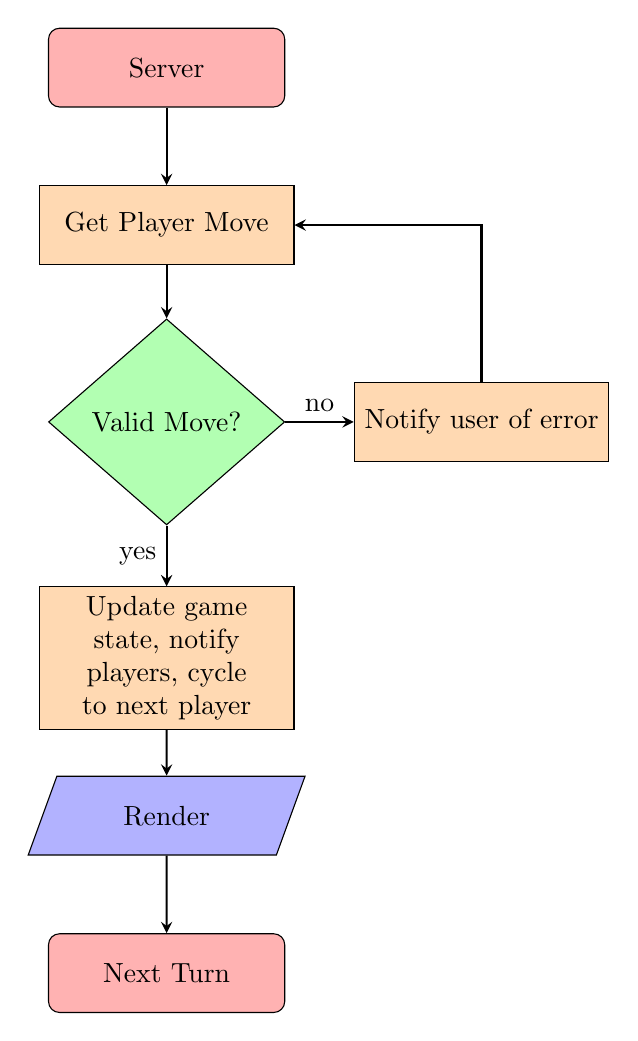
\begin{tikzpicture}[node distance=2cm]
    \node (server) [startstop] {Server};
    \node (pro1) [process, below of=server] {Get Player Move};
    \node (dec1) [decision, below of=pro1, yshift=-0.5cm] {Valid Move?};
    \node (pro2a) [process, below of=dec1, yshift=-1.0cm] {Update game state, notify players, cycle to next player};
    \node (pro2b) [process, right of=dec1, xshift=2cm] {Notify user of error};
    \node (out1) [io, below of=pro2a] {Render};
    \node (stop) [startstop, below of=out1] {Next Turn};

    \draw [arrow] (server) -- (pro1);
    \draw [arrow] (pro1) -- (dec1);
    \draw [arrow] (dec1) -- node[anchor=east] {yes} (pro2a);
    \draw [arrow] (dec1) -- node[anchor=south] {no} (pro2b);
    \draw [arrow] (pro2b) |- (pro1);
    \draw [arrow] (pro2a) -- (out1);
    \draw [arrow] (out1) -- (stop);
    \end{tikzpicture}
    \caption{Game Move Validation Logic}
    \label{fig:diagrams_gmvl}
\end{figure}

\subsubsection{External Interface}
\label{sec:fun_reqs_server_external}

The interface players and spectators will see displays basic
information such as whose turn it is, board state and the valid
move of the current player as well as  any notifications that
the players need to see. 

\subsection{Client Functionality}
\label{sec:fun_reqs_client}
This section details the functions that the clients will be
responsible for during a standard execution of the game of
checkers. The clients are further broken into two cases being
the player client and the spectator client. 

\subsubsection{Player}
\label{sec:fun_reqs_client_normal}

\begin{enumerate}
    \item \textbf{Connect to server}

          The client shall attempt to make a TCP connection to
          the server on a specified port. Once a connection has
          been established the client will enter a
          \texttt{listening} state in which it listens for data
          from the server to begin a game.
          
    \item \textbf{Initial connection fails}

          In the event a connection to the server fails, the
          client will inform the player that a connection issue
          occurred, and attempt to connect again. After a
          specified number of failed attempts, the client will
          inform the user that a connection cannot be
          established, and the client will close.
          
    \item \textbf{Receive board state from server}

          The client will accept the board state as part of the
          data communication format shown in 
          \cref{fig:fun_reqs_server_gamestate_struct}
          
    \item \textbf{Display board state to player}
          
          The client will display the board, described in
          \cref{sec:ui_game_board}
          
    \item \textbf{Handle case where server disconnects}
          
          In the event that the server disconnects prematurely,
          defined as:
          \begin{enumerate}
            \item the network connection is dropped for any
                reason
          \end{enumerate}
          The client will notify the player in the form of
          a \textbf{Game State Message}, described in
          \cref{sec:ui_game_messages}
          
    \item \textbf{Receive messages from server}
          
          The client will accept messages as part of the
          data communication format shown in
          \cref{fig:fun_reqs_server_gamestate_struct}
          
    \item \textbf{Display messages to player}
          
          The client will display messages as
          \textbf{Action Messages}, described in
          \cref{sec:ui_game_messages}.
          
    \item \textbf{Get move from player}
          
          In the event the server requests a move from the
          client, the client enters a \texttt{move selection}
          state. The client utilizes the user interface
          described in \cref{sec:ui_game_move} to get a
          move. If a jump is made, additional jumps are
          checked.
          
    \item \textbf{Player refuses to move}
          
          Please refer to \cref{sec:fun_reqs_server_client}.
          
    \item \textbf{Validate move}
          
          Once the player selects a move sequence the client
          will check the validity of the move. Should the
          move be found invalid, it is rejected, and a new
          move is requested from the player.
          
    \item \textbf{Send move to server}
          
          The valid move sequence is sent to the server
          using the data communication format shown in
          \cref{fig:fun_reqs_server_gamestate_struct}
          
    \item \textbf{Display winner to player}
          
          The client will display the winner as a
          \textbf{Game State Message}, described in
          \cref{sec:ui_game_messages}.
          
    \item \textbf{Restart match at user request}
          
          The client will query both active players, to
          determine if they want to start a new game.
          
\end{enumerate}

\subsubsection{Spectator}
\label{sec:fun_reqs_client_spectator}

\textbf{Like in \cref{sec:fun_reqs_client_normal}, except}:

\begin{enumerate}
    \item Spectators cannot make any moves or in any way
          communicate with the other players
    \item If a spectator is disconnected for any reason, the two
          normal clients shall continue gameplay uninterrupted
    \item No clients or spectators shall be notified upon the
          disconnection of any spectator
    \item The server does not wait for any input from the
          spectator
\end{enumerate}

%---------------------------------------------------------------
% Non-Functional Requirements.

\section{Non-Functional Requirements}
\label{sec:nofun_reqs}

\subsection{Performance}
\label{sec:nofun_reqs_performance}

\subsubsection{Server}

The server software must be able to handle the following:

\begin{enumerate}
    \item \textbf{Receive frequent messages from remote client}
          
          Connected clients will send move sequences as
          requested by the server
          
    \item \textbf{Send frequent messages to remote client}
          
          The server will send the board state to all
          connected clients, as well as request moves from
          the designated client's turn
          
    \item \textbf{Validate a given move in reasonable time}
          
          The server will evaluate a move sequence provided
          by a client, containing at least one move but
          possibly a sequence of moves comprising a sequence
          of jumps.
          
\end{enumerate}

\subsubsection{Client}

The client software must be able to handle the following:

\begin{enumerate}
    \item \textbf{Receive frequent messages from remote server}
          
          The client will accept the board state, move request,
          and messages, in the format shown in 
          \cref{fig:fun_reqs_server_gamestate_struct}.
          
    \item \textbf{Send frequent messages to remote server}
          
          The client will send move sequences to the server
          when requested by the server
          
    \item \textbf{Validate a given move in a reasonable time}
          
          Before sending a move sequence to the server, the
          client will evaluate the move sequence, consisting
          of at least one move but possible a sequence of
          moves comprising a sequence of jumps.
          
\end{enumerate}

\subsection{Safety}
\label{sec:nofun_reqs_safety}

This program shall not be able to move any physical devices, to 
prevent damage to the system, users, or surroundings. It shall
also be free of memory leaks, so it does not compromise the
systems that it is being run on.

\subsection{Security}
\label{sec:nofun_reqs_security}

In order to keep relative security of the integrity of the
software, both the client and server shall validate moves that
are input by the user.

\subsection{Software Quality}
\label{sec:nofun_reqs_quality}

Both the server and client software shall be implemented using
a set of standards that is agreed upon by all developers. This
shall keep code standardized for other developers to maintain.

\subsection{Limitations}
\label{sec:nofun_reqs_limitations}

Unless explicitly defined in this document, no additional
features or functionality should be implemented.

%---------------------------------------------------------------
% Other Requirements.

\section{Other Requirements}
\label{sec:other}

We make the assumption that the terminal window is at least
\texttt{80x24} columns, with the preferred size being at least
\texttt{150x50} columns.

%---------------------------------------------------------------
% User Interface.

\section{User Interface}
\label{sec:ui}

\subsection{Initialization Screen}
\label{sec:ui_initial}

The initialization screen will be shown to the user when their
client is launched, changing to the game screen once a game
begins. This screen will display the game logo, as well as a
message detailing the current task the client is performing:

\begin{enumerate}
    \item Connecting to server
    \item Waiting for game
\end{enumerate}

\subsection{Game Screen}
\label{sec:ui_game}

The game screen is shown the duration of the game, until the
client closes. This screen will display the board to the user,
showing the board itself and the checker pieces. It will also
display messages to the user, and facilitate move selection.
The size of the display will be dynamically sized based on
the size of the terminal.

\subsubsection{Board}
\label{sec:ui_game_board}

The board will be displayed as a grid filling a majority of
the terminal of color alternating between red and white,
with bottom-left and top-right spaces being red. We avoid
using black because the standard terminal is also black,
which could confuse the user.

\subsubsection{Pieces}
\label{sec:ui_game_pieces}

The pieces will be displayed as letters:

\begin{enumerate}
    \item Basic - \textbf{C}
    \item King - \textbf{K}
\end{enumerate}

The letters will be colored according to the player they
belong to. Should time permit, the pieces will be made
to be colored circles, with the crowned pieces having a
crown icon to distinguish them from the standard pieces.

\subsubsection{Move Facilitation}
\label{sec:ui_game_move}

\begin{enumerate}
    \item The game screen will use highlighting to denote which
          pieces are capable of being selected for a move,
          placed on the inside border of the grid square
    \item Selected pieces will have a blinking highlight in the
          same location as above highlighting
    \item The left and right arrow keys will be used to switch
          which piece is selected, moving the blinking
          highlight
    \item The \texttt{enter} key will confirm the selection
\end{enumerate}

\subsubsection{Messages}
\label{sec:ui_game_messages}

          Strings (of messages) are encoded in the general data
          structure that the server sends to clients with the
          current game state, etc. Clients should passively
          receive these messages, displaying them to the player.
          Messages will be handled in two different ways,
          depending on the priority of the message.

\begin{enumerate}
    \item \textbf{Action Messages (Notifications)}
          
          Messages relating to actions required of the player
          should be displayed above the board, at the top of
          the screen, not disrupting gameplay. Messages shall
          remain on the screen until a new message is to be
          displayed, overwriting the previous.
          
          \begin{enumerate}
              \item You must perform a jump
              \item Another jump is available
          \end{enumerate}
          
    \item \textbf{Game Status Messages}
    
          Messages relating the the state of the game should
          be overlayed on top of the board. These messages
          will require the \texttt{enter} key be pressed to
          acknowledge and close the message.
          
          \begin{enumerate}
              \item Player Red is the winner!
              \item Player White has disconnected
              \item A Draw has been reached
          \end{enumerate}
          
\end{enumerate}

%---------------------------------------------------------------
% Use Cases.

\section{Use Cases}
\label{sec:usecases}

\subsection{Joining a game}
\label{sec:usecases_joining}

Running the client, while an accessible server is running on
the port that the client is directed at will cause the client
to connect. Once two clients have connected, they will be placed
into a game together.\\

\prepost
{A server is being run on an accessible network}
{A handshake occurs}
{The server and client have established a connection}

\subsection{Making a move}
\label{sec:usecases_move}

A player selects the \textbf{C} piece they would like to move
from the list of pieces that have the ability to move. All
possible moves become highlighted once a piece is selected. They
then select the destination of that piece, based on available
valid moves. The \textbf{C} pieces have the ability to move
forward along the diagonals of the board.\\

\prepost
{At least one piece has valid move}
{Player selects a piece, and its destination}
{The piece is moved to the destination and the board is updated
for all players}

\subsection{Crowning a piece}
\label{sec:usecases_king}

A piece becomes a King when the player successfully moves it to
a space along the border of the board, on the opposite side from
where the piece started the game.\\

\prepost
{A piece has a valid move that places it against the border of
the board, on the opposite side from where it started the game}
{Player selects that piece to move and the border location as
its destination}
{The piece is moved to the destination and transforms from a
\textbf{C}, to a \textbf{K}, while remaining the color
associated with the player that owns it. The board is then
updated for all players}

\subsection{Moving a King}
\label{sec:usecases_moveking}

A player selects the \textbf{K} piece that they would like to
move from the list of pieces that have the ability to move. All
possible moves become highlighted once a piece is selected. They
then select the destination of that piece, based on available
valid moves. The \textbf{K} pieces have the ability to move
forward or backward along the diagonals of the board.\\

\prepost
{At least one piece has valid move}
{Player selects a piece, and its destination}
{The piece is moved to the destination and the board is updated
for all players}

\subsection{Jumping a piece}
\label{sec:usecases_jump}

If it is possible for a piece to jump an opposing piece, that
move must be taken. The opposing piece that is jumped is then
removed from the game.\\

\prepost
{A piece has a valid move involving performing a jump}
{Player selects that piece to move and the location that it
would finish its jump as the destination}
{The piece is moved to the destination and the opposing piece
that was jumped is removed from the game. The board is then
updated for all players}

\subsection{Multi-Jumping}
\label{sec:usecases_multijump}

If it is possible for a piece to jump an opposing piece, that
jump must be made. If the same piece is able to jump another
opposing piece from the end location of the first jump, that
jump must also be made. A piece may make any number of such
jumps per turn. All of the opposing pieces that are jumped are
then removed from the game.\\

\prepost
{A piece has finished at least one jump during its turn, and
is positioned such that another jump would be a legal move}
{Player confirms the mandatory jump}
{The piece is moved to the destination and the opposing piece
that was jumped is removed from the game. The board is then
updated for all players. This process is then repeated, if
possible}

\subsection{Winning the game}
\label{sec:usecases_winning}

To win the game, the player must remove all of their opponents
pieces from the board, or force them into a situation where they
can not make a legal move. Once either state is reached, the
game is over, and the players may start a new match.\\

\prepost
{The game is in progress}
{A player removes all of the opponent's pieces from the game, 
or forces the opponent into a situation where they are unable
to make a legal move}
{The game ends, and the server sends a message to both players
declaring the winner to be the player. Both players are queried
to see if a rematch will be played}

\subsection{Losing the game}
\label{sec:usecases_losing}

If all of the players pieces are removed from the game, the
player has lost, and the game is over. Once this state is
reached, the game is over, and the players may start a new
match.\\

\prepost
{The game is in progress}
{The current player has all their pieces removed from the board}
{The game ends, and the server sends a message to both players
declaring the winner to be the opponent. Both players are
queried to see if a rematch will be played}

\subsection{Unable to move piece}
\label{sec:usecases_immobile}

If a player is unable to move a piece on their turn the game
will end with them losing. Once this state is reached, the game
is over, and the players may start a new match.\\

\prepost
{The game is in progress}
{The opponent makes the current player unable to move}
{The game ends, and the server sends a message to both players
declaring the winner to be the opponent. Both players are
queried to see if a rematch will be played}

\subsection{Playing a rematch}
\label{sec:usecases_rematch}

Once a game has been completed, both active players will be
asked if they would like to play again. If both players agree,
the game state is reset, and play restarts. If one player does
not agree, and there are spectators present, the specatators
shall be asked if they would like to join, in the order in which
they connected, until either a new game is created, or the list
of spectators is exhausted.\\

\prepost
{The game has ended, with any outcome}
{Both players agree to play another game}
{The game is reset, and play restarts as a new game, with the
same active players and spectators}

%---------------------------------------------------------------
% Glossary.

\newpage

\section{Glossary}
\label{sec:glossary}

\begin{itemize}
    \item \textbf{Checkerboard} NxN (typically 8x8) game board
          composed of alternating white/red (or other) squares
          on which game pieces \emph{Checkers} reside
    \item \textbf{Piece} Standard Checkers piece with limited
          movement, specifically only forward-diagonal motion
    \item \textbf{King} Checkers piece that can move along any
          diagonals, forward or backward
    \item \textbf{Move} the act of changing the location of a
          piece on the board when it is that player's turn
    \item \textbf{Jump} the act of removing an opposing player's
          piece from the board, occurring in a straight diagonal
          fashion -- e.g., ``hopping over'' the opponent
    \item \textbf{Multi-jump} the act of chaining multiple 
          \emph{Jumps} together, with one piece, in a single
          turn
    \item \textbf{Crowning} the act of changing a standard game
          piece to a \emph{King}
\end{itemize}

\newpage

%---------------------------------------------------------------
% References.

%\addcontentsline{toc}{chapter}{References}
\renewcommand{\bibsection}{\section{\refname}} % uses natbib

\begin{thebibliography}{9}

\bibitem{draughts}
    Wikipedia, \emph{Draughts},
    online at\\
    \url{https://en.wikipedia.org/wiki/Checkers}

\bibitem{ieeesrs}
    IEEE Computer Society, \emph{29148-2011 - ISO/IEC/IEEE
    International Standard - Systems and software engineering --
    Life cycle processes -- Requirements engineering}
    
\bibitem{webassembly}
    Haas, A., et al.,
    \emph{Bringing the Web up to Speed with WebAssembly},
    DOI: http://dx.doi.org/10.1145/3062341.3062363\\
    online at\\
    \url{https://github.com/WebAssembly/spec/raw/master/papers/pldi2017.pdf}

\bibitem{vnc}
    Martin, J. et al., \emph{noVNC: HTML5 VNC Client},
    online at\\
    \url{https://github.com/novnc/noVNC}

\bibitem{rules}
    The Spruce, \emph{How to Play Checkers: Standard U.S. Rules},
    online at\\
    \url{https://www.thespruce.com/play-checkers-using-standard-rules-409287}

\bibitem{docker}
    Docker Inc., \emph{Docker}, available online at\\
    \url{https://www.docker.com/}

\bibitem{musl}
    Felker, Rich, et al., \emph{musl},
    online at\\
    \url{https://www.musl-libc.org/}

\bibitem{ncurses}
    Free Software Foundation, Inc., \emph{ncurses},
    online at\\
    \url{https://www.gnu.org/software/ncurses/ncurses.html}

\bibitem{check}
    Malec, A., et al., \emph{Check: A Unit Testing Framework for C},
    online at\\
    \url{https://libcheck.github.io/check/}

\bibitem{freetype}
    Turner, D., Wilhelm, R., et al., \emph{FreeType},
    online at\\
    \url{https://www.freetype.org/}

\bibitem{cppcheck}
    Marjamäki, D., \emph{Cppcheck},
    online at\\
    \url{http://cppcheck.sourceforge.net/}

\bibitem{valgrind}
    The Valgrind Developers, \emph{Valgrind},
    online at\\
    \url{http://valgrind.org/}

\end{thebibliography}

%---------------------------------------------------------------
% Document end.

\end{document}